\section{Análise do Problema}
\label{sec:prob}

Como mencionado no Trabalho 1, a inSoft é uma empresa júnior da Universidade de Brasília (UnB) fundada em agosto de 2015 por alunos do curso de Engenharia de Software da Faculdade do Gama (FGA). Sendo uma empresa júnior, seu objetivo é o de criar um ambiente para estudantes aplicarem os conhecimentos aprendidos em aula desenvolvendo soluções em software que agregem valor e ajudem a sociedade, retornando uma parte do investimento que é depositado no ensino público à sociedade.

Por ser uma empresa nova, os processos da inSoft são instáveis e ainda em elaboração, funcionando de forma ad hoc, o que evidencia a necessidade de definir e melhorar os seus processos.

Em um primeiro momento, através de sessões de brainstorming, a equipe de MPR nos transmitiu o fishbone de problemas de negócio, que mensurava os problemas da empresa em um todo, como:

\begin{itemize}
  \item \textbf{Grande número de partes interessadas:}
  O alto número de partes interessadas burocratiza a empresa e cria uma clara dificuldade de comunicação, mais atrapalhando do que agregando valor à empresa e impactando diretamente os seus projetos.
\end{itemize}


\begin{itemize}
  \item \textbf{Falta de visibilidade de horários/habilidades de cada membro:}
  A falta de visibilidade de horários, e habilidades específicas de cada membro da equipe, dificulta a designação de desenvolvedores para um determinado projeto, gerando uma sobrecarga no Diretor de Desenvolvimento.
\end{itemize}

\begin{itemize}
  \item \textbf{Ordenação ruim de ativides:}
  Quando a empresa, consegue determinado projeto, o ordenação de atividades dentro do projeto é ruim, onde não há alocações especifícas de desenvolvedores e de responsáveis por cada tarefa.
\end{itemize}

\begin{itemize}
  \item \textbf{Processo informal:}
  Como dito anteriormente, a empresa funciona de maneira ad hoc, não possuindo um processo formal ou bem definido, consequentemente, a equipe não tem visibilidade do processo, e isso acarreta problemas tanto na negociação de projetos, como na parte de desenvolvimento.
\end{itemize}

	Sendo assim, todos esse fatores ou causas, acarretam em um problema maior que é o fato da empresa nunca ter conclúido um projeto.

  \begin{figure}[H]
    \center
    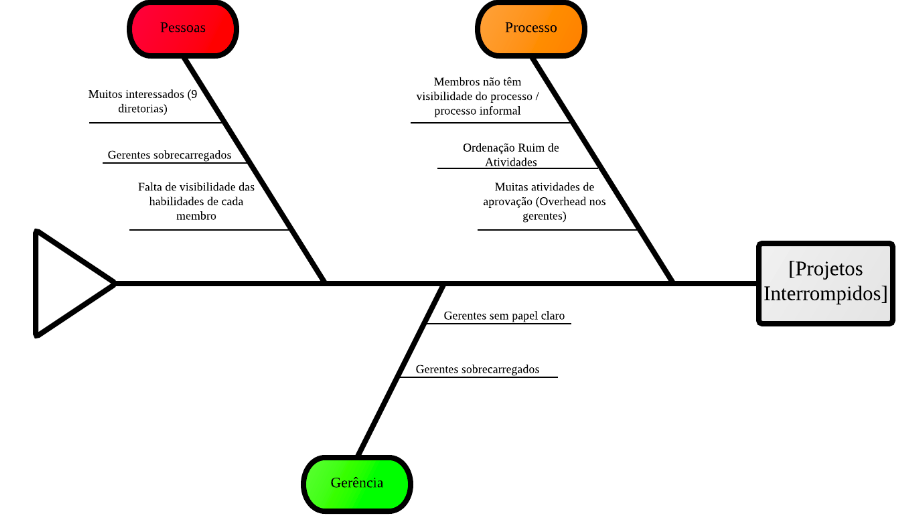
\includegraphics[width=1.0\textwidth]{figuras/fishbone-mpr}
    \caption{Fishbone Problemas de Negócio}
    \label{fig:fishbone_mpr}
  \end{figure}



  Após o entendimento dos problemas como um todo, a equipe de MPR fez uma priorização dos processos e designou que nossa área de atuação seria o desenvolvimento. Então, a partir do fishbone de problemas de negócio, foi priorizado os problemas que poderiam ser solucionados com software, e que estavam relacionados ao desenvolvimento, e então foi gerado o fishbone de problemas de desenvolvimento, afim de identificar fatores e causas que contribuíam para os problemas decorrentes da área de desenvolvimento.

  \begin{figure}[H]
    \center
    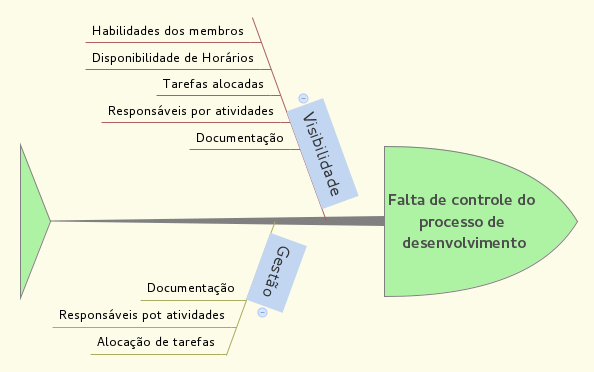
\includegraphics[width=0.7\textwidth]{figuras/fishbone-requisitos}
    \caption{Fishbone Problemas de Desenvolvimento}
    \label{fig:fishbone_requisitos}
  \end{figure}

  Como visto no fishbone acima, dentro do processo de desenvolvimento da empresa, a falta de visibilidade de habilidades especificas e horários disponíveis de cada membro, assim como a gestão da documentação e de alocação de tarefas e seus responsáveis, são causas que contribuem para um problema maior que é a falta de controle do processo de desenvolvimento. Abaixo, temos a descrição do problema:



    \begin{table}[H]
        \centering
        \begin{tabular}{|>{\columncolor[HTML]{C0C0C0}}p{0.26\textwidth}|p{0.65\textwidth}|}
          \hline
          O problema de         &   falta de controle do processo de desenvolvimento \\ \hline
          afeta                 &   toda a equipe de desenvolvimento                 \\ \hline
          cujo impacto é        &   a desorganização da equipe de desenvolvimento;
                                    o desconhecimento das tarefas a serem executadas pela equipe;
                                    a demora na execução dos projetos de desenvolvimento e eventual cancelamento dos mesmos                                         \\ \hline
          uma boa solução seria &   desenvolver um sistema em \emph{software} que possibilite:
                                    disponibilizar todas as informação dos membros relevantes para o desenvolvimento;
                                    gerenciar múltiplos projetos de desenvolvimento;
                                    gerenciar as tarefas de desenvolvimento de cada projeto;
                                    \\ \hline
        \end{tabular}
        \caption{Descrição do Problema da inSoft}
      \end{table}



      Sendo assim, tem-se como tarefa uma solução para o problema descrito, afim de melhorar o processo de desenvolvimento da empresa como um todo, para que futuramente a empresa consiga atender vários projetos simultaneamentes, e consequentemente evoluir no mercado.
